\documentclass[conference]{IEEEtran}

\usepackage{cite}
\usepackage{amsmath,amssymb,amsfonts}
\usepackage{algorithm}
\usepackage{algpseudocode}   % NOT \usepackage{algorithmic}
\usepackage{graphicx}
\usepackage{textcomp}
\usepackage{xcolor}
\usepackage{booktabs}
\usepackage{siunitx}

\def\BibTeX{{\rm B\kern-.05em{\sc i\kern-.025em b}\kern-.08em
    T\kern-.1667em\lower.7ex\hbox{E}\kern-.125emX}}

\begin{document}

\title{System Level Energy and Cost Characterization of Hybrid Quantum–Classical Cloud Workloads}

\author{
\IEEEauthorblockN{1\textsuperscript{st} Waylon Luo}
\IEEEauthorblockA{\textit{Kent State University} \\
Kent, OH, USA}
\and
\IEEEauthorblockN{2\textsuperscript{nd} Joao Vitor Macambira Donaton}
\IEEEauthorblockA{\textit{Kent State University} \\
Kent, OH, USA}
\and
\IEEEauthorblockN{3\textsuperscript{rd} Priyabrata Senapati}
\IEEEauthorblockA{\textit{Kent State University} \\
Kent, OH, USA}
\and
\IEEEauthorblockN{4\textsuperscript{th} Qiang Guan}
\IEEEauthorblockA{\textit{Kent State University} \\
Kent, OH, USA}
}

\maketitle

\begin{abstract}

% WORD COUNT LIMIT 150. 

Near-term quantum workloads depend on hybrid quantum-classical cloud architectures, yet their power and performance dynamics remain difficult to characterize. To address this, we present a high-level simulation framework to evaluate power, energy, and cost across heterogeneous QPU and CPU clouds. By modeling macro level interactions such as job arrivals, workflow iterations, and device power states, the framework orchestrates administrative-level evaluation without requiring detailed quantum properties. To demonstrate the framework with selected configurations and workload, we sweep the variational iteration count over a fixed fleet, holding circuit width, depth, shots, and arrival patterns constant, so that loop length serves as the sole independent variable. While the classical phase scales linearly, the quantum phase departs abruptly from linearity beyond a critical iteration count. Energy, cost, and turnaround time escalate rapidly, and turnaround per job becomes heavily tailed because nearly all quantum phase time is spent blocked on qubit connectivity rather than computing.

\end{abstract}

\begin{IEEEkeywords}
Quantum cloud simulations, quantum job scheduling, Hybrid-cloud simulation frameworks
\end{IEEEkeywords}

\section{Introduction}
\label{sec:introduction}

In recent years, quantum computing has transitioned from a theoretical concept~\cite{feynman2018simulating} to a rapidly maturing technology that garners academic research~\cite{gracejohnson2022} and industrial interest. According to the MIT Quantum Index Report 2025 \cite{ruane2025quantum}, the field is experiencing an unprecedented expansion in hardware availability, corporate communications, and global intellectual property, evidenced by a fivefold increase in quantum technology patents over the past decade. The rapid development of commercial Quantum Processing Units (QPUs) highlights the urgent need for hybrid infrastructure capable of orchestrating classical and quantum workloads.

\begin{figure*}[h]
    \centering
    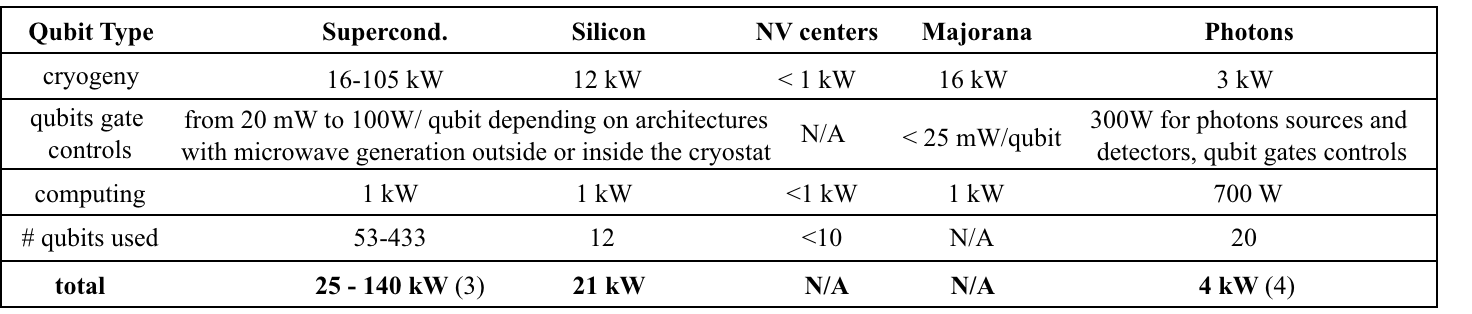
\includegraphics[width=\textwidth]{Images/energy_usage-compact.png}
    \caption{Energetic requirements and architectural comparison of quantum computing modalities (source: Ezratty et al.~\cite{ezratty2021}).}
    % \Description{}
    \label{fig:energy_usage}
\end{figure*}

However, raw quantum advantage cannot be realized in isolation. Modern quantum algorithms, such as the Variational Quantum Eigensolver (VQE)~\cite{peruzzo2014vqe}, Quantum Approximate Optimization Algorithm (QAOA), and Quantum Neural Networks (QNNs), are inherently hybrid. These workloads depend on tight feedback loops where classical High Performance Computing (HPC) nodes handle statevector simulation, parameterized circuit compilation, and numerical optimization, while the QPUs execute quantum state preparations and measurements. As a result, the ultimate system throughput is constrained not only by QPU fidelity or qubit counts, but also by the efficient orchestration, dynamic scheduling, and data transfer overheads between classical CPU resources and heterogeneous QPU coprocessors.

This work is motivated by the need to model and quantify energy and power consumption within hybrid quantum cloud architectures. Because physical hardware access is constrained and energy dynamics in hybrid environments are complex, simulation serves as a vital tool. It allows researchers and system architects to model complex execution workflows, test scheduling hypotheses, and predict performance and energy metrics across scale. To bridge this critical tooling gap, this paper leverages HybridCloudSim, a discrete event simulation framework engineered to model, evaluate, and optimize hybrid classical quantum cloud environments. HybridCloudSim connects algorithmic specifications and physical hardware dynamics by establishing capacity aware models for both CPU clusters and QPU hardware pools. 

Our contributions in this paper are as follows:

\textbf{Unified resource scheduling and brokerage.} A broker that schedules concurrent, heterogeneous jobs under strict capacity constraints, allocating CPU cores and memory bandwidth classically while resolving quantum allocation at two levels, namely aggregate qubit capacity and physical connectivity, so that fragmentation effects invisible to qubit count only models are exposed.

\textbf{Energy and power accounting.} A configurable cost model that attributes energy per execution phase from device specific power profiles drawn from Ezratty et al.~\cite{ezratty2021} as the ground truth.

\textbf{Integrated telemetry and monitoring.} An event driven monitor that records device utilization, instantaneous fleet power, and queueing behavior at event boundaries, producing traces that support analysis over the run itself rather than end of run aggregates.

Through a series of simulation studies, we demonstrate how HybridCloudSim enables system architects to locate hardware bottlenecks, compare dynamic scheduling policies, and reason about the energy and cost implications of resource allocation in emerging hybrid cloud infrastructures. In particular, we show that energy and power aware simulation provides a principled basis on which researchers and cloud operators can set pricing policy, by varying device configurations and workload parameters within the framework rather than by procuring physical hardware. This work demonstrates that simulation models can assist researchers and cloud administrators in establishing pricing based on energy and power consumption by adjusting parameters and configurations directly within the framework. Detailed circuit execution is deliberately abstracted away, allowing the framework to act as a lightweight digital twin of a hybrid quantum classical cloud. As this work targets orchestration level modeling, we refer the reader to Nielsen and Chuang~\cite{nielsen2010quantum} for a detailed introduction to quantum computation and quantum information theory.

\section{Related Work}
\label{sec:related-work}

Classical cloud simulators, such as CloudSim~\cite{calheiros2011cloudsim}, iCanCloud~\cite{nunez2012icancloud}, and SimGrid~\cite{casanova2008simgrid}, are designed to evaluate resource management and scheduling without physical infrastructure~\cite{jawaddi2024gymcloudsim}. Many of these foundational tools have been extended to support specific operational needs; for example, WorkflowSim~\cite{chen2012workflowsim} adds complex scientific workflow modeling, while frameworks like GreenCloud~\cite{kliazovich2012greencloud} and E-mc$^2$~\cite{castane2013emc2} introduce formal energy modeling for data centers~\cite{makaratzis2018energymodeling}. Collectively, they demonstrate the utility of discrete event simulation for analyzing system dynamics and computational accounting.

As quantum computing increasingly adopts a cloud-based delivery model dedicated simulation toolkits have arisen to model hybrid quantum environments. Frameworks such as iQuantum~\cite{nguyen2024iquantum}, QSimPy~\cite{qsimpy2024, nguyen2024drlq}, and QCloudSim~\cite{luo2025digital} apply discrete event simulation to evaluate quantum task scheduling, backend selection, and resource management strategies. 

While simulation frameworks are critical for exploring these emerging architectures, existing quantum cloud simulators~\cite{Jones2019-nc, Brennan2022QXToolsAJ, diadamo2021qunetsim} focus primarily on performance, resource allocation, and queueing. They generally lack explicit energy and cost estimation at the workflow level. Furthermore, many frameworks~\cite{bian2023pas, fan2021drascqsim} treat quantum jobs as monolithic, overlooking the interleaved QPU and CPU execution phases central to hybrid algorithms.

Prior work shows that practical quantum overhead is driven by workload traits, backend variability, repeated sampling, and classical-quantum interactions. Senapati et al.~\cite{senapati2023reproducibility} showed hardware calibration drift degrades workload reproducibility across backends. Related research characterized noise-sensitive states~\cite{senapati2023visualization,senapati2025noisy} and devised predictive NISQ backend selection for quantum machine learning~\cite{senapati2024pqml}. Subsequent uncertainty quantification studies analyzed execution variability, stability, and backend selection for variational quantum algorithms and VQE~\cite{senapati2025uqvarqa,senapati2026vqe}. Additional work across hybrid molecular simulation~\cite{abraham2026manybody}, machine learning translation~\cite{zeng2026qbridge}, and variational/signal processing workloads~\cite{senapati2026unified} confirms that total execution cost is determined by the end-to-end hybrid workflow---including iterative classical optimization, repeated executions, and backend choice---rather than isolated quantum circuits.

Energy consumption is a critical concern in high performance computing (HPC)~\cite{Veigas2025, iea2025data_centers}, driving interest in quantum computing as a potentially energy efficient complement~\cite{martin2022energy, jaschke2023quantum}. While classical supercomputers can consume hundreds of megawatt-hours daily, present day quantum processors operate in the kilowatt range. However, meaningful energy evaluation requires analyzing total system power integrated over execution time, as a quantum computer's footprint is dictated by its supporting infrastructure rather than gate level operations. As summarized in Figure~\ref{fig:energy_usage}~\cite{ezratty2021}, superconducting systems demand significantly more power due to their environmental control requirements than other quantum systems.

In superconducting platforms, energy consumption is overwhelmingly dominated by system level infrastructure. Total system power ranges from 25~kW to over 140~kW, depending on system configuration and qubit count~\cite{ezratty2021}. The primary contributor is the cryogenic refrigeration required to maintain millikelvin temperatures, drawing between 16~kW and 105~kW. Additional components, such as classical computing overhead and qubit gate control electronics, contribute marginally (often around 1~kW) and are generally subsumed into the total system consumption.

Based on this observation, we developed an energy accounting model in which the energy consumed by a quantum job is proportional to the duration for which it occupies QPUs and CPUs. Under this abstraction, the energy consumption of a superconducting quantum job is approximated as $E_{\text{job}} \approx P_{\text{baseline}} \cdot t_{\text{occupy}}$, where \(P_{\text{baseline}}\) denotes the average system-level power consumption, including cryogenics and supporting electronics, and \(t_{\text{occupy}}\) represents the job's execution interval on the quantum device. This baseline power model aligns with energy accounting practices commonly used in HPC systems, where always-on infrastructure costs are amortized over job execution time. 
\section{System Architecture}
\label{sec:architecture}

HybridCloudSim is a discrete event simulator built on SimPy. It models a hybrid cloud at the \emph{orchestration} layer: job arrival, device selection, capacity blocking, iterative quantum classical execution, and the resulting energy and cost. Circuit level quantum behavior is deliberately abstracted; device service times are obtained from analytical performance models parameterized by published hardware specifications, so that a full run over thousands of jobs completes in seconds on a single core.

\subsection{Overview}
\label{sec:arch-overview}

\begin{figure}[t]
\centering
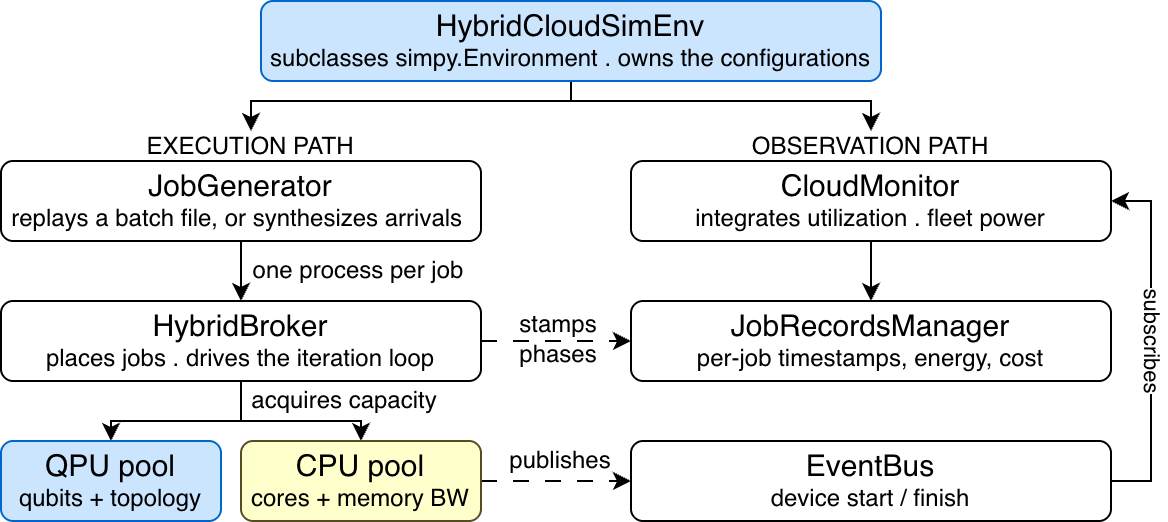
\includegraphics[width=0.99\linewidth]{Images/architecture.png}
\caption{Component structure of HybridCloudSim. Both paths descend from the composition root, but they never join: the execution path (left) places jobs and consumes device capacity, while the observation path (right) only records what the execution path has already committed. Dashed links carry telemetry and never influence placement.}
\label{fig:architecture}
\end{figure}

The simulation framework is organized around a single composition root, \texttt{HybridCloudSimEnv}, which subclasses the SimPy environment and instantiates every other component. Table~\ref{tab:components} summarizes the roles. Control flows top down, where the job feed creates one broker process per job, and each broker drives devices. Observability flows bottom up: devices emit events on a publish subscribe bus and write per job records that the monitor and the records manager aggregate.

\begin{table}[t]
\centering
\caption{Principal components of HybridCloudSim.}
\label{tab:components}
\small
\begin{tabular}{@{}ll@{}}
\toprule
\textbf{Component} & \textbf{Responsibility} \\
\midrule
\texttt{HybridCloudSimEnv} & Composition root; owns the cost model \\
\texttt{JobGenerator}      & Trace replay or stochastic arrivals \\
\texttt{HybridBroker}      & Per job scheduling and phase control \\
\texttt{QuantumDevice}     & Qubit capacity, topology, QPU time \\
\texttt{CPU}               & Core and memory bandwidth capacity \\
\texttt{EventBus}          & Decoupled device event notification \\
\texttt{CloudMonitor}      & Utilization integration, fleet power \\
\texttt{JobRecordsManager} & Event log, and job metrics \\
\bottomrule
\end{tabular}
\end{table}

A run is fully specified by three inputs: a device inventory (a list of QPU and CPU objects), a workload (a trace file or an arrival process), and a cost configuration. Devices are constructed detached from the environment and are bound to it in a separate initialization pass, at which point their SimPy containers and resources are created. This two phase construction keeps device definitions declarative and makes parameter sweeps explicit: because devices carry mutable state, specifically qubit containers, the topology graph, and the qubit occupancy map, a fresh inventory is instantiated for each configuration in a sweep. 

Figure~\ref{fig:architecture} makes this separation explicit. The execution and observation paths descend from the same root but never join: the broker consults device capacity in order to place work, whereas the event bus, the cloud monitor, and the records manager only ever read state that the execution path has already committed. No scheduling decision depends on a telemetry value. This asymmetry is what allows instrumentation to be as dense as the analysis requires; every phase transition of every job is stamped, and every device transition is published, without perturbing the schedule under study. It also fixes the provenance of each reported quantity: phase boundaries originate in the broker, device arrivals in the devices themselves, time integrated utilization and instantaneous fleet power in the monitor, and per job energy and cost in the records manager. We rely on that provenance in Section~\ref{sec:arch-telemetry}, where the two independently computed energy figures are reconciled.

\subsection{Workload}
\label{sec:arch-workload}

A job is a tuple
$J=(n, d, s, p, a, r, c, b)$
giving qubit count $n$, circuit depth $d$, shot count $s$, priority $p$, arrival time $a$, required iterations $r$, CPU units $c$, and memory bandwidth $b$. Jobs enter the system in one of two modes. In \emph{dispatcher} mode the generator replays a CSV or JSON trace, releasing each job at its recorded arrival time; this is the mode used for all experiments in this paper, since it makes workloads reproducible and shareable. In \emph{generator} mode jobs are synthesized online from a configurable inter arrival distribution (exponential by default) with randomized circuit parameters. In both modes the generator spawns one broker process per job, so concurrency in the model is bounded by device capacity rather than by any fixed pool of workers.

\subsection{Broker and Execution Lifecycle}
\label{sec:arch-broker}

The broker is the scheduling core. Each job executes $r$ variational iterations, and every iteration consists of a QPU phase followed by a CPU phase, reflecting the structure of VQE and QAOA style workloads in which measurement outcomes are returned to a classical optimizer that produces the next parameter set. Algorithm~\ref{alg:broker} states the loop.

\begin{algorithm}[t]
\caption{Broker process for job $J$}
\label{alg:broker}
\begin{algorithmic}[1]
\State $i \gets 0$
\While{$i < r$}
  \State $q \gets \Call{Select}{\mathrm{QPU}, n}$
  \While{$q = \mathrm{null}$} \Comment{no device has free capacity}
    \State \textbf{wait} $\delta$;\quad $q \gets \Call{Select}{\mathrm{QPU}, n}$
  \EndWhile
  \State \Call{Execute}{$q$, $J$};\quad \Call{Record}{$J$, QPU}
  \State $u \gets \Call{Select}{\mathrm{CPU}, (c,b)}$
  \While{$u = \mathrm{null}$}
    \State \textbf{wait} $\delta$;\quad $u \gets \Call{Select}{\mathrm{CPU}, (c,b)}$
  \EndWhile
  \State \Call{Execute}{$u$, $J$};\quad \Call{Record}{$J$, CPU}
  \State $i \gets i + 1$
\EndWhile
\State \Call{FinalizeEnergyAndCost}{$J$}
\end{algorithmic}
\end{algorithm}

\textsc{Select} filters the inventory to devices of the requested type that are not under maintenance and whose free capacity meets the request, namely free qubits for a QPU, free cores \emph{and} free memory bandwidth for a CPU, and returns the most lightly loaded candidate, breaking ties in favor of the device with the largest residual capacity. When no candidate exists the broker retries after a fixed polling interval $\delta$ rather than enqueueing, which keeps the admission decision re-evaluated against current fleet state. The resulting blocking behavior, rather than an explicit queue discipline, is what produces the contention observed in Section~\ref{sec:use-cases}. The policy is localized in \textsc{Select}, so alternative disciplines (priority, fair share, energy aware placement) can be substituted without touching the phase loop.

\section{Models}
\label{sec:models}

We adopt an energy accounting model inspired by practices in HPC~\cite{beloglazov2012energy}. Electrical energy consumption is defined as the time integral of instantaneous power consumption,
\[
E = \int_{t_s}^{t_e} P(t)\,dt,
\]
where \(P(t)\) denotes the system power draw and \([t_s, t_e]\) represents the execution interval of a job.

For superconducting quantum computers, system power is dominated by the cryogenic refrigeration and supporting infrastructure required to operate continuously and maintain qubit coherence \cite{matsumoto2024}. However, while this baseline cooling requirement is massive, the total power consumption is not strictly independent of workload characteristics \cite{ueno2025}. We approximated instantaneous power consumption as constant during operation,
\[
P(t) \approx P_{\text{baseline}}.
\]

Under this assumption, the energy consumption of a quantum job simplifies to
\[
E_{\text{job}} \approx P_{\text{baseline}} \cdot (t_e - t_s),
\]
where \(P_{\text{baseline}}\) assumes the average power consumption, including cryogenics, control electronics, and classical infrastructure.

This accounting model simplifies energy attribution without relying on fine-grained gates or pulses, which are difficult to obtain and validate for current quantum hardware. 

The parameters used to model energy consumption in this experiment are summarized in Table~\ref{tab:qcloudsim_energy_params}. Given these parameters, the energy consumption of a quantum job is computed as
\[
E_{\text{job}} = \frac{P_{\text{baseline}} \cdot t_{\text{compute}}}{N_{\text{concurrent}}},
\]
where $N_{\text{concurrent}} = 1$ for exclusive access devices. This formulation accounts for potential time sharing or concurrent execution scenarios without altering the underlying energy model.

Each job consists of a sequence of execution stages that alternate between QPU and CPU devices. For a given job $j$, execution on QPUs and CPUs is recorded as ordered lists of start and finish timestamps:

\[
\{\texttt{qpu\_start}_i^j,\texttt{qpu\_finish}_i^j\}_{i=0}^{N_q-1}
\]
\[
\{\texttt{cpu\_start}_i^j,\texttt{cpu\_finish}_i^j\}_{i=0}^{N_c-1}
\]

where $N_q$ and $N_c$ denote the number of QPU and CPU execution segments, respectively.  

Each QPU segment corresponds to a quantum execution phase, while each CPU segment represents classical pre-processing, post-processing, or intermediate computation required by the hybrid algorithm.

The window $\texttt{qpu\_finish}_i^j - \texttt{qpu\_start}_i^j$ of the $i$-th QPU segment also contains the time the job spends waiting for a connected qubit region (Section~\ref{sec:arch-qpu}); it is retained as the segment's occupancy, while the execution time billed for energy is the circuit execution time recorded by the device,
\[
t^{\text{qpu}}_i = \texttt{qpu\_compute}_i^j,
\]
and the execution time of the $i$-th CPU segment is
\[
t^{\text{cpu}}_i = \texttt{cpu\_finish}_i^j - \texttt{cpu\_start}_i^j.
\]

In that way, quantum and classical execution phases are interleaved multiple times within a single job.

\begin{table}[t]
\centering
\caption{Energy related parameters for superconducting quantum devices}
\label{tab:qcloudsim_energy_params}
\begin{tabular}{llp{5cm}}
\toprule
\textbf{Parameter} & \textbf{Unit} & \textbf{Description} \\
\midrule
$P_{\text{baseline}}$ & kW & Average power consumption, including cryogenic refrigeration, control electronics, and classical infrastructure. \\
$t_{\text{compute}}$ & h & Circuit execution time of a quantum job on the quantum processing unit, excluding time spent waiting for a connected qubit region. \\
$E_{\text{job}}$ & kWh & Energy consumption attributed to an individual quantum job. \\
$N_{\text{concurrent}}$ & -- & Number of concurrently executing jobs sharing the device (if supported). \\
\bottomrule
\end{tabular}
\end{table}

\subsection{Two-Level QPU Allocation}
\label{sec:arch-qpu}

QPUs are the sole spatially constrained resource in the model. Each device loads a topology graph $G=(V,E)$ ($|V|$ physical qubits) and maintains a qubit occupancy map. Admission requires a two-level check: (1) an aggregate counter showing at least $n$ free qubits, and (2) a breadth-first search confirming a \emph{connected} induced subgraph of $n$ free qubits. Upon allocation, selected qubits are marked busy and their adjacent edges cut; upon completion, qubits are freed and cut edges restored between available pairs.

Unlike capacity-only abstractions, this two-level model captures qubit fragmentation: a job meeting the aggregate threshold can still fail admission if free qubits are disconnected, reflecting multi-tenant behavior on sparsely connected superconducting lattices.


QPU service time follows a throughput model based on the vendor-reported Circuit Layer Operations Per Second (CLOPS) metric:

\begin{equation}
\label{eq:qpu-time}
t_{\mathrm{QPU}} \;=\; \alpha\,\frac{M K S \log_2 d}{\mathrm{CLOPS}},
\end{equation}
where $S$ is the shot count, $d$ the circuit depth, $M$ and $K$ the number of circuit templates and parameter updates per submission, and $\alpha$ a unit conversion constant. Per-device calibration tables (readout, single-qubit, and two-qubit gate errors) are additionally loaded to expose an estimated circuit fidelity alongside timing, though fidelity does not feed back into scheduling in the present study. 

\subsection{Classical Device Model}
\label{sec:arch-cpu}

Classical nodes expose two independent capacities, compute units and memory bandwidth, both of which must be satisfied for a job to be admitted; modeling bandwidth separately is necessary because statevector post-processing is frequently bandwidth- rather than compute-bound. The default node derives its service time from the algorithmic cost of the classical half of the variational loop:

\begin{equation}
\label{eq:cpu-time}
t_{\mathrm{CPU}} \;=\; \frac{\kappa\, 2^{\,n} d\, \pi}{\eta\, c^{\,0.85}},
\qquad
\eta = \tfrac{1}{2}\bigl(f_{\mathrm{base}} + f_{\mathrm{boost}}\bigr)\cdot\mathrm{IPC},
\end{equation}

where $\pi$ is the variational parameter count, $\kappa$ a calibration constant, $\eta$ the effective per-core throughput derived from clock and IPC, and the exponent $0.85$ captures sublinear scaling with allocated units. The $2^{\,n}$ term makes the classical side of the loop grow exponentially with qubit width, which is the mechanism by which classical post-processing overtakes quantum execution as circuits widen. A simpler node with randomized service time is also provided for baseline comparisons.

\subsection{Energy and Cost Model}
\label{sec:arch-energy}

Power parameters are set via a single environment configuration with per-device overrides. QPUs draw constant power $P^q$ (dominated by load-independent cryogenic cooling) whenever hosting a job, while classical nodes follow an affine power model based on utilization $u_j$. Instantaneous fleet power is:
\begingroup
\small
\begin{equation}
\label{eq:power}
P(t) \;=\; \sum_{q \in \mathcal{Q}} P^{q}\,\mathbb{1}\!\left[\text{$q$ busy at $t$}\right]
\;+\; \sum_{j \in \mathcal{C}} \Bigl[P^{j}_{\mathrm{idle}} + \bigl(P^{j}_{\mathrm{peak}} - P^{j}_{\mathrm{idle}}\bigr) u_j(t)\Bigr].
\end{equation}
\endgroup

Per-job energy is attributed by phase. For job $J$ with QPU computation times $t^{q}_{i}$ and CPU phase durations $t^{c}_{i}$ on the devices selected in iteration $i$,
\begin{equation}
\label{eq:energy}
E(J) \;=\; \sum_{i=1}^{r}\Bigl(P^{q}_{i} t^{q}_{i} + P^{c}_{i} t^{c}_{i}\Bigr),
\qquad
\mathrm{Cost}(J) \;=\; \rho\, E(J),
\end{equation}
with $\rho$ the electricity price per kWh. Equations~\eqref{eq:power} and~\eqref{eq:energy} are complementary rather than redundant: the former gives the operator's instantaneous load, which determines provisioning and peak demand charges, while the latter gives the per-tenant attribution needed to set prices. Both are driven by the same configuration, so a change to a device's power profile propagates to both views.

\subsection{Telemetry}
\label{sec:arch-telemetry}

Devices stream \texttt{device\_start} and \texttt{device\_finish} events. On each event, the cloud monitor integrates resource-time metrics to record exact utilization and power~\eqref{eq:power}. Exact event-boundary sampling scales with system activity rather than wall-clock time. Concurrently, a records manager logs timestamps to track latency and compute final makespan, energy, and cost~\eqref{eq:energy}. Storing per-iteration traces supports both cross-job and within-job analysis. Aggregated job energy is compared with the integrated power series, which measures fleet occupancy rather than per tenant computation and is not expected to match it.



\section{System Metrics: Instantaneous vs. Cumulative Utilization}
\label{sec:instant_vs_cumulative}

To evaluate the operational efficiency and temporal dynamics of the hybrid quantum-classical cloud scheduler, we distinguish between \textit{instantaneous resource load} and \textit{cumulative resource utilization}. While instantaneous load measures real-time demand variations and queue drainage, cumulative utilization captures the time-integrated efficiency of the heterogeneous hardware over the entire operational lifespan of the simulation.

\subsection{System Capacity Definitions}
Let $\mathcal{D}_{\text{QPU}}$ and $\mathcal{D}_{\text{CPU}}$ represent the sets of quantum processing units (QPUs) and classical central processing units (CPUs), respectively. The static global capacity of each resource type is defined as:
\begingroup
\small
\begin{equation}
    C_{\text{QPU}} = \sum_{d \in \mathcal{D}_{\text{QPU}}} c(d), \quad 
    C_{\text{CPU}} = \sum_{d \in \mathcal{D}_{\text{CPU}}} c(d), \quad 
    C_{\text{MEM}} = \sum_{d \in \mathcal{D}_{\text{CPU}}} b(d)
\end{equation}
\endgroup
where $c(d)$ denotes the resource unit capacity (e.g., qubits or core counts) of device $d$, and $b(d)$ represents the associated memory bandwidth capacity.

\subsection{Instantaneous Resource Load}
At any given simulation time $t \in [0, T]$, the instantaneous load $L_{k}(t)$ for a resource type $k \in \{\text{QPU}, \text{CPU}, \text{MEM}\}$ measures the fraction of hardware capacity actively committed to processing workloads. Let $u_k(t)$ be the total units of resource $k$ allocated at time $t$. The instantaneous load percentage is defined as:
\begin{equation}
    L_{k}(t) = \left( \frac{u_k(t)}{C_k} \right) \times 100\%
\end{equation}

When the job queue depletes and all active workloads complete at time $t_{\text{idle}} \le T$, the active allocation drops to zero ($u_k(t) = 0$), yielding:
\begin{equation}
    \lim_{t \to t_{\text{idle}}^+} L_{k}(t) = 0\%
\end{equation}
Thus, $L_{k}(t)$ is non-monotonic and exhibits sharp step-wise transitions corresponding to job arrivals and completions.

\subsection{Cumulative Resource Utilization}
Whereas instantaneous load evaluates active demand at a discrete millisecond, cumulative utilization $U_{k}(T)$ quantifies total resource consumption relative to total available resource-time product over the entire elapsed simulation window $[0, T]$. 

The cumulative workload metric is formulated as the integral of active unit allocations over time:
\begin{equation}
    W_k(T) = \int_{0}^{T} u_k(t) \, dt
\end{equation}

The total available resource capacity integrated across time $T$ is given by:
\begin{equation}
    \Omega_k(T) = C_k \cdot T
\end{equation}

The cumulative percentage utilization $U_k(T)$ up to time $T$ is therefore expressed as:
\begin{equation}
    U_k(T) = \left( \frac{W_k(T)}{\Omega_k(T)} \right) \times 100\% = \left( \frac{\int_{0}^{T} u_k(t) \, dt}{C_k \cdot T} \right) \times 100\%
\end{equation}

\subsection{Discrete Event Formulation}
In a discrete-event simulation paradigm (such as SimPy), state transitions occur at discrete timestamps $t_0, t_1, t_2, \dots, t_N$. The continuous integral $W_k(T)$ is evaluated exactly via zero-order hold accumulation across intervals $\Delta t_i = t_i - t_{i-1}$:
\begin{equation}
    W_k(T) = \sum_{i=1}^{N} u_k(t_{i-1}) \cdot (t_i - t_{i-1})
\end{equation}

Unlike instantaneous load $L_k(t)$, the cumulative utilization $U_k(T)$ does not drop abruptly to zero upon workload completion. Instead, if the system remains idle beyond $t_{\text{idle}}$, $W_k(T)$ remains constant while the denominator $\Omega_k(T)$ grows linearly with $T$, causing $U_k(T)$ to exhibit a smooth, asymptotic decay toward zero:
\begin{equation}
    U_k(T) = \left( \frac{W_k(t_{\text{idle}})}{C_k \cdot T} \right) \times 100\%, \quad \forall \, T \ge t_{\text{idle}}
\end{equation}

\section{Use Cases}
\label{sec:use-cases}

We design a representative use case that reflects workload heterogeneity, resource contention, and energy cost interactions across quantum and classical subsystems. 

We generate a synthetic workload consisting of 1,200 independent quantum circuit synthesis jobs, stored in a CSV file and submitted to the simulator as an external job trace. 

\begin{table}[t]
\centering
\caption{HybridCloudSim Use Case Configurations and Workload Parameters}
\label{tab:use-case-summary}
\begin{tabular}{p{0.31\linewidth} p{0.60\linewidth}}
\hline
\textbf{Category} & \textbf{Configuration} \\
\hline
Workload size & 1,200 hybrid synthesis jobs (CSV trace) \\

Quantum workload parameters &
\begin{tabular}[t]{@{}l@{}}
Number of qubits: 10 to 25 \\
Circuit depth: 37 to 99 \\
Shots per job: 1,000 to 5,000 \\
Iterations per job: 4 to 9 \\
Arrival process: Exponential ($\lambda \approx 0.36$)
\end{tabular} \\

Classical workload parameters &
\begin{tabular}[t]{@{}l@{}}
CPU units: 4 to 7 (qubit scaled) \\
Memory BW units: 4 to 7 (qubit scaled)
\end{tabular} \\

Quantum resources &
\begin{tabular}[t]{@{}l@{}}
2 $\times$ IBM Eagle r3 QPUs (127 qubits each) \\
IBM\_Quebec: 32,000 CLOPS \\
IBM\_Kyiv: 30,000 CLOPS
\end{tabular} \\

Classical resources &
\begin{tabular}[t]{@{}l@{}}
1 $\times$ CPU nodes \\
8 cores, 16 threads per node \\
Base / boost: 3.8 / 5.0 GHz \\
Memory bandwidth: 51.2 GB/s
\end{tabular} \\

Resource abstraction &
\begin{tabular}[t]{@{}l@{}}
CPU capacity = threads $\times$ cpu units \\
Mem BW capacity = GB/s $\times$ mem units
\end{tabular} \\

Energy pricing & \$0.18 per kWh \\

QPU power model &
\begin{tabular}[t]{@{}l@{}}
Static power draw: 50 kW each\\
\end{tabular} \\

CPU power model &
\begin{tabular}[t]{@{}l@{}}
Per job billing: constant at peak \\
CPU peak: 5.0 kW \\
Fleet power: affine, idle 30\% of peak
\end{tabular} \\

\hline
\end{tabular}
\end{table}

Table~\ref{tab:use-case-summary} summarizes the characteristics of the workload, infrastructure, and cost configuration used in our hybrid quantum classical cloud simulation. This consolidated view is intended to improve reproducibility and provide readers with a concise overview of the experimental setup. Here, \textit{cpu units} and \textit{memory units} represent normalized per thread compute capacity and per GB/s bandwidth capacity, respectively. The trace's classical columns are recorded but not consulted by the dispatcher: as in Section~\ref{sec:iter-setup}, every CPU phase is admitted against a fixed budget of 8 CPU and 20 memory bandwidth units.

We assume a fixed electricity price of \$0.18 per kWh, representative of commercial cloud pricing. Quantum devices are modeled with static power draw values to reflect the high baseline energy cost of superconducting systems, with each QPU assigned a power draw of 50 kW. These values are selected within the reported power consumption range of superconducting quantum computing systems~\cite{ezratty2021}.

A classical CPU node is assigned a device specific power envelope of 5.0\,kW, at which each job is billed for the duration of its own computation, while the node's instantaneous draw in the fleet view follows an affine model between an idle floor of 30\% of that envelope and the envelope itself. We note that absolute CPU power values are less critical in our study, as our results are driven by the relative energy imbalance between QPU and classical resources. The detailed models are provided in Section~\ref{sec:models}.

\subsection{Performance Evaluation}
\label{sec:performance-evaluation}

In this section, we evaluate the performance characteristics of the HybridCloudSim environment setup and analyze aggregate cloud resource usage to understand overall system behavior, followed by a time series analysis to capture temporal utilization dynamics.

In terms of cost, the mean energy cost per job is \$0.099556 $\pm$ 0.049350, with a median cost of \$0.0939 and a 95th percentile cost of \$0.190520, reflecting the right skewed cost distribution. Energy fraction statistics further confirm the dominant role of quantum execution, with a mean QPU energy fraction of 0.981943 $\pm$ 0.079422 and a mean CPU energy fraction of 0.018050 $\pm$ 0.079423. These results quantitatively reinforce the earlier observation that overall energy consumption and cost in hybrid quantum classical workloads are overwhelmingly driven by QPU operation, while classical resources contribute smaller but non negligible overheads.

\subsection{Time Series Resource Utilization}
\label{subsec:time-series-utilization}

\begin{figure}[t]
    \centering
    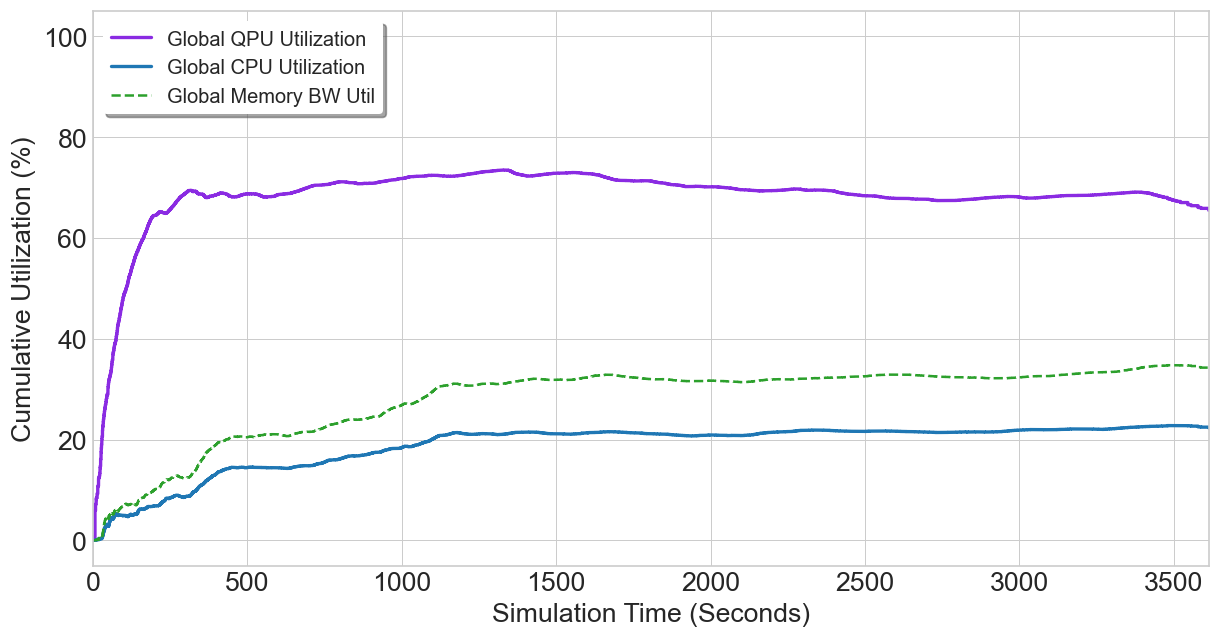
\includegraphics[width=0.99\linewidth]{Images/Performance/Cloud-utilization.png}
    \caption{Cumulative Cloud Resource Utilization Over Time.}
    \label{fig:cumulative_utilization}
\end{figure}

Figure~\ref{fig:cumulative_utilization} illustrates the cumulative time integrated resource utilization across the hybrid quantum cloud environment over a 3,764 second execution window. During the initial warm up phase ($t < 500\,\text{s}$), all three subsystem resources experience a steep ramp up in utilization as arriving workloads fill the system pipelines. The global quantum processing unit (QPU) utilization rises rapidly, stabilizing into a steady state regime between $67\%$ and $73\%$ between $t = 500\,\text{s}$ and $t = 3,500\,\text{s}$. This sustained high demand highlights the QPU as the primary performance bottleneck within the hybrid infrastructure. In contrast, classical resource demands stabilize at lower levels, with memory bandwidth cumulative utilization settling between $30\%$ and $35\%$ after $t \approx 1{,}200\,\text{s}$ and global CPU utilization settling near $20\%$ to $23\%$. The pronounced gap between QPU and CPU or memory utilization reflects the asymmetric nature of quantum classical workflows, where classical hardware spends significant time idle while waiting for long duration quantum circuit executions to complete. The detailed calculations are provided in Section~\ref{sec:instant_vs_cumulative}.

\subsection{Energy Consumption and Cost Analysis}
\label{subsec:energy-analysis}

We next analyze the energy characteristics of the hybrid quantum classical cloud environment. 

\subsubsection{Distribution of Energy Cost Across Jobs}

\begin{figure}[t]
    \centering
    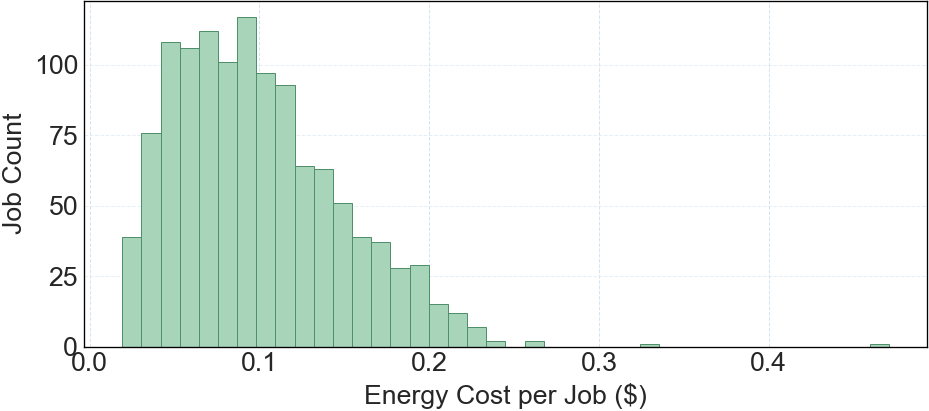
\includegraphics[width=0.99\linewidth]{Images/Performance/Energy-cost-distribution.png}
    \caption{Distribution of energy cost per job (\$) across executed workloads, showing a right-skewed distribution where the majority of jobs incur costs under \$0.20, with a small tail extending up to \$0.48.}
    \label{fig:energy-cost-distribution}
\end{figure}

Figure~\ref{fig:energy-cost-distribution} shows the distribution of energy cost per job, computed using the modeled energy consumption and a fixed electricity price. The distribution is right skewed, with most jobs clustered at lower costs and a diminishing number of higher cost outliers.

This behavior arises from variability in circuit depth, qubit count, execution duration, and iterative workload structure. Importantly, the absence of multimodal behavior suggests that cost variation is driven by continuous workload heterogeneity rather than discrete execution regimes. 

\subsubsection{Time Series Power Consumption}

\begin{figure}[t]
    \centering
    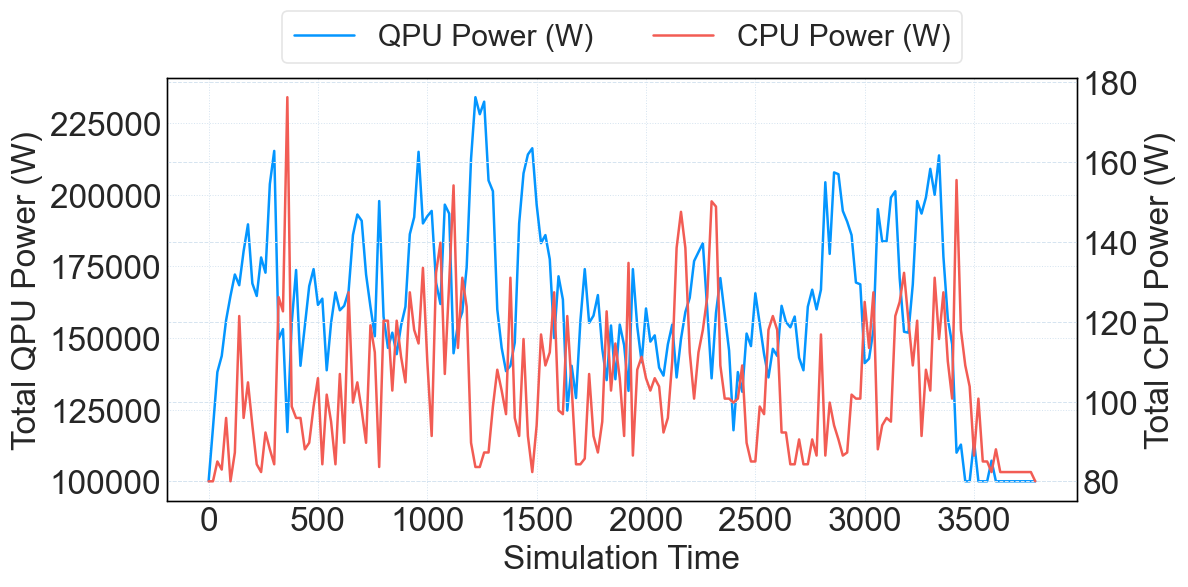
\includegraphics[width=0.99\linewidth]{Images/Performance/Power-timeseries.png}
    \caption{Time-series profile of QPU (left y-axis, blue) and CPU (right y-axis, red) power consumption in Watts over total simulation time (seconds) under the load dependent power variant described in the text, illustrating the dynamic resource utilization and power fluctuations during hybrid quantum-classical execution.}
    \label{fig:power-timeseries}
\end{figure}

Figure~\ref{fig:power-timeseries} illustrates the time series power consumption of QPU and CPU resources. It is drawn from the job records by an illustrative load dependent variant of the power model rather than by Eq.~\eqref{eq:power}: the two QPUs draw their combined 100~kW baseline rising linearly toward 300~kW with the fraction of a fixed 640 qubit reference capacity claimed by admitted jobs, each counted from admission to release, and the CPU node draws 80~W rising toward 360~W with the 1.3 power of its unit utilization. Because admitted jobs are counted before a connected region is secured, the claimed fraction measures demand pressure on the fleet rather than physical qubit occupancy, and under contention it exceeds what 254 qubits could hold. The QPU power remains persistently high, fluctuating within a range of approximately 100{,}000 to 235{,}000~W around its baseline operating level. These variations coincide with active execution periods, but they sit on top of a fixed 100~kW cryogenic cooling and control baseline that the two QPUs draw even when idle, which alone accounts for over 60\% of the 160~kW mean draw.

In contrast, CPU power operates at a significantly lower scale on this variant's 80 to 360~W envelope, distinct from the 5.0~kW billing rate, varying between roughly 80 and 175~W over time. Unlike the QPU, CPU power exhibits more pronounced relative fluctuations that correlate with classical execution phases, job arrivals, and orchestration activities. This stark separation in power magnitude between QPU and CPU resources indicates that energy optimization in hybrid quantum classical environments is primarily driven by QPU utilization efficiency rather than classical compute scaling.

As shown in Fig.~\ref{fig:energy_usage}, the plotted series spans an aggregate QPU power draw of approximately 100 to 235~kW for a configuration consisting of two superconducting QPUs, corresponding to roughly 50 to 117~kW per QPU. We note that these results are contingent on the chosen configuration parameters, taking Ezratty et al.~\cite{ezratty2021} as the baseline reference. Modifying the system or workload inputs will naturally alter the simulation outcomes. This sensitivity is a key advantage of our highly configurable framework.

\section{Hybrid Workflow Behavior}
\label{sec:hybrid-workflow-behavior}

Many near term quantum applications are realized not as single shot quantum programs, but as \emph{iterative hybrid quantum classical workflows}. Representative examples include the Variational Quantum Eigensolver (VQE), the Quantum Approximate Optimization Algorithm (QAOA), and hybrid calibration and tuning routines deployed in contemporary quantum cloud environments.

To isolate the impact of hybrid workflow structure on system behavior, we conduct a controlled experiment in which physical resources, circuit characteristics, and workload composition are held constant, while only the number of quantum classical iterations per job is varied.

\begin{table}[t]
\centering
\caption{Simulation Configuration and Workload Characteristics for hybrid workflow behavior.}
\label{tab:use-case-2-summary}
\begin{tabular}{p{0.31\linewidth} p{0.60\linewidth}}
\hline
\textbf{Category} & \textbf{Configuration} \\
\hline
Workload size & 3,000 synthesis jobs  \\

Quantum workload parameters &
\begin{tabular}[t]{@{}l@{}}
Number of qubits: 10 to 20 \\
Circuit depth: 10 to 20 \\
Shots per job: 2,000 to 9,000 \\
Arrival process: Exponential ($\lambda \approx 1.04$)
\end{tabular} \\

Classical workload parameters &
\begin{tabular}[t]{@{}l@{}}
CPU units: 7 to 10 (qubit scaled) \\
Memory BW units: 14 to 20 (qubit scaled)
\end{tabular} \\

Quantum resources &
\begin{tabular}[t]{@{}l@{}}
2 $\times$ QPUs \\
IBM\_Strasbourg (127 qubits) \\
IBM\_Brussels (127 qubits)
\end{tabular} \\

Classical resources &
\begin{tabular}[t]{@{}l@{}}
2 $\times$ CPU nodes \\
8 cores, 16 threads per node \\
Base / boost: 3.8 / 5.0 GHz \\
Memory bandwidth: 51.2 GB/s
\end{tabular} \\

Resource abstraction &
\begin{tabular}[t]{@{}l@{}}
CPU capacity = threads $\times$ cpu units \\
Mem BW capacity = GB/s $\times$ mem units
\end{tabular} \\

Energy pricing & \$0.18 per kWh \\

QPU power model &
\begin{tabular}[t]{@{}l@{}}
Static power draw \\
QPU 1: 70 kW \\
QPU 2: 60 kW
\end{tabular} \\

CPU power model &
\begin{tabular}[t]{@{}l@{}}
Affine utilization based model \\
CPU 1 peak: 5.0 kW \\
CPU 2 peak: 6.5 kW
\end{tabular} \\

\hline
\end{tabular}
\end{table}

The experimental setup is listed in Table~\ref{tab:use-case-2-summary}. We use a fixed set of 3,000 synthesized quantum jobs generated with identical distributions for qubit counts, circuit depth, shot count, and classical resource requirements. The hybrid environment consists of two QPUs and two CPU devices, operated under the same scheduling policy and cost model parameters across all experimental runs.

The sole parameter that differs between experiments is the required number of hybrid iterations per job. Specifically, we evaluate seven workflow configurations with iteration counts ranging from 3 to 21 in increments of 3. Each configuration is provided as a separate workload trace. The purpose is to assure that any observed differences in execution time, energy consumption, or cost are attributable exclusively to changes in workflow structure rather than hardware variability or workload diversity.

\subsection{Iteration Scaling and the Onset of Quantum Congestion}
\label{sec:iteration-scaling}

Variational algorithms (e.g., VQE, QAOA) iteratively alternate between $k$ circuit execution rounds and classical parameter updates. Standard hybrid cloud cost models assume a linear multiplier where $k$ iterations cost $k\times$ a single iteration; the assumption holds only for the computation itself. Beyond a critical iteration count, the time a job occupies a QPU per iteration escalates by more than an order of magnitude while its computation, and the classical phase, scale perfectly linearly. This effect stems from contention across a finite quantum fleet rather than from the application; it is invisible to models that ignore device occupancy and misattributed by those that bill the occupied window as computation.


\subsection{Experimental Design}
\label{sec:iter-setup}

The experiment is a single factor sweep. We generate one batch of $N=3000$ synthetic variational jobs and replicate it seven times, altering exactly one field, namely the requested iteration count $k \in \{3,6,9,12,15,18,21\}$. Every other job attribute is bit identical across the seven traces: qubit width, circuit depth, shot count, priority, arrival timestamp, CPU core demand, and memory bandwidth demand. Any difference in the measured outcome is therefore attributable to $k$ alone, with no confounding from workload composition or arrival pattern.

Jobs request $10$ to $20$ qubits (mean $15.15$), circuit depth $10$ to $20$, $2000$ to $9000$ shots (mean $5501$), $7$ to $10$ CPU units, and $14$ to $20$ memory bandwidth units. Arrivals are replayed over a window of $2884.8$ simulation seconds, a mean rate $\lambda \approx 1.04$ jobs per second. The classical columns are not consulted: every CPU phase is admitted against a fixed budget of $8$ CPU and $20$ memory bandwidth units and runs on a CPU unit allocation drawn uniformly from $4$ to $16$, the sweep's sole stochastic element.

The target platform is a fixed hybrid inventory: two superconducting QPUs modeled on IBM Eagle r3 devices (\texttt{IBM\_Strasbourg} as QPU 1 and \texttt{IBM\_Brussels} as QPU 2, $127$ physical qubits each on the heavy hex coupling map, with their published CLOPS, quantum volume, and $T_1/T_2$ figures), and two \texttt{AMDRyzen} classical nodes, instantiated afresh for every run so that no qubit occupancy or topology state leaks between configurations. Energy is attributed per phase from constant device draws of \qty{70}{\kilo\watt} (QPU 1), \qty{60}{\kilo\watt} (QPU 2), \qty{5.0}{\kilo\watt} (CPU 1), and \qty{6.5}{\kilo\watt} (CPU 2) at $\$0.18$ per \unit{\kilo\watt\hour}. Each configuration runs to completion and is summarized over all $3000$ jobs.

Two structural features of the platform matter for what follows. First, a QPU admits several jobs concurrently, bounded not by a job slot count but by free qubits: at a mean width of $15.15$ qubits, the $254$ qubit fleet could in principle host $C \approx 16.8$ jobs at once. Second, admission is resolved at two levels, specifically aggregate qubit capacity \emph{and} physical connectivity. A job is admitted only when a \emph{connected} subgraph of free qubits exists, so the achievable concurrency is strictly below $C$ whenever the free qubits are scattered across the coupling graph.

It is convenient to summarize the concurrency demand by the dimensionless ratio
\begin{equation}
  \rho(k) \;=\; \frac{\lambda \, s_1 \, k}{C},
  \label{eq:rho}
\end{equation}
where $s_1 = \qty{0.971}{\second}$ is the QPU computation time of a single iteration, identical at every sweep point. Equation~\eqref{eq:rho} is the fraction of nominal fleet concurrency that the workload demands; it rises from $\rho = 0.18$ at $k=3$ to $\rho = 1.26$ at $k=21$ and passes unity at $k \approx 16.6$.

\subsection{Metrics and Figure Construction}
\label{sec:iter-metrics}

For each QPU phase the device records its \emph{computation} time $T_{\mathrm{comp}}$, the circuit execution time of Eq.~\eqref{eq:qpu-time}, while the broker stamps its \emph{occupancy} $T_{\mathrm{occ}}$, the window from admission at the capacity gate to release, throughout which the job is resident on a powered device; they differ by the time spent retrying the connectivity check of Section~\ref{sec:arch-qpu}, once per second, until a connected free region exists. Per job energy is charged on $T_{\mathrm{comp}}$ alone; it is the QPU phase duration entering Eq.~\eqref{eq:energy}. Since Eq.~\eqref{eq:qpu-time} depends only on job attributes, $\sum T_{\mathrm{comp}}$ is linear in $k$ \emph{by construction}: a control, not a finding. Figure~\ref{fig:iteration-knee} therefore reports three \emph{derived}, scale free views of the sweep, each chosen so that the linear scaling null hypothesis appears as a flat line and departure from linearity as departure from flatness.

\paragraph{Panel (a): computation and occupancy per iteration.}
We divide the mean per job QPU computation, QPU occupancy, and CPU phase time by $k$, the average cost of one iteration on each resource class. Under the multiplier assumption all three series are horizontal. All three share one logarithmic axis (\unit{\second} per iteration) because occupancy spans a factor of $41$ while the other two do not move.

\paragraph{Panel (b): compute fraction of occupied QPU time.}
For each run we form the ratio of sums
\begingroup
\small
\begin{equation}
  \eta \;=\; \frac{\sum T_{\mathrm{comp}}}{\sum T_{\mathrm{occ}}} \;\in\; (0, 1],
  \label{eq:eta}
\end{equation}
\endgroup
the fraction of reserved, powered QPU time that performs computation. $\eta = 1$ is exactly the multiplier assumption and serves as the reference; a second line at $\eta = \tfrac12$ marks the point past which most occupied QPU time is idle.

\paragraph{Panel (c): dispersion and tail weight.}
We plot two dimensionless descriptors of the per job turnaround distribution \emph{within} each run: the coefficient of variation $\mathrm{CV} = \sigma/\mu$, and the tail ratio $p_{95}/\mathrm{median}$. Both are invariant to the overall time scale, so they isolate changes in the \emph{shape} of the distribution from changes in its magnitude. The reference line at $\mathrm{CV}=1$ marks exponential like dispersion, the canonical signature of a queue that has begun to build.

In all three panels a shaded band marks the congested regime, its left edge where $\eta$ falls through one half, interpolated inside the $12 \to 15$ bracket ($k \approx 13$). The figure is generated from the sweep summary by \texttt{plot\_iteration\_knee.py} without smoothing or fitting.


\begin{figure*}[t]
  \centering
  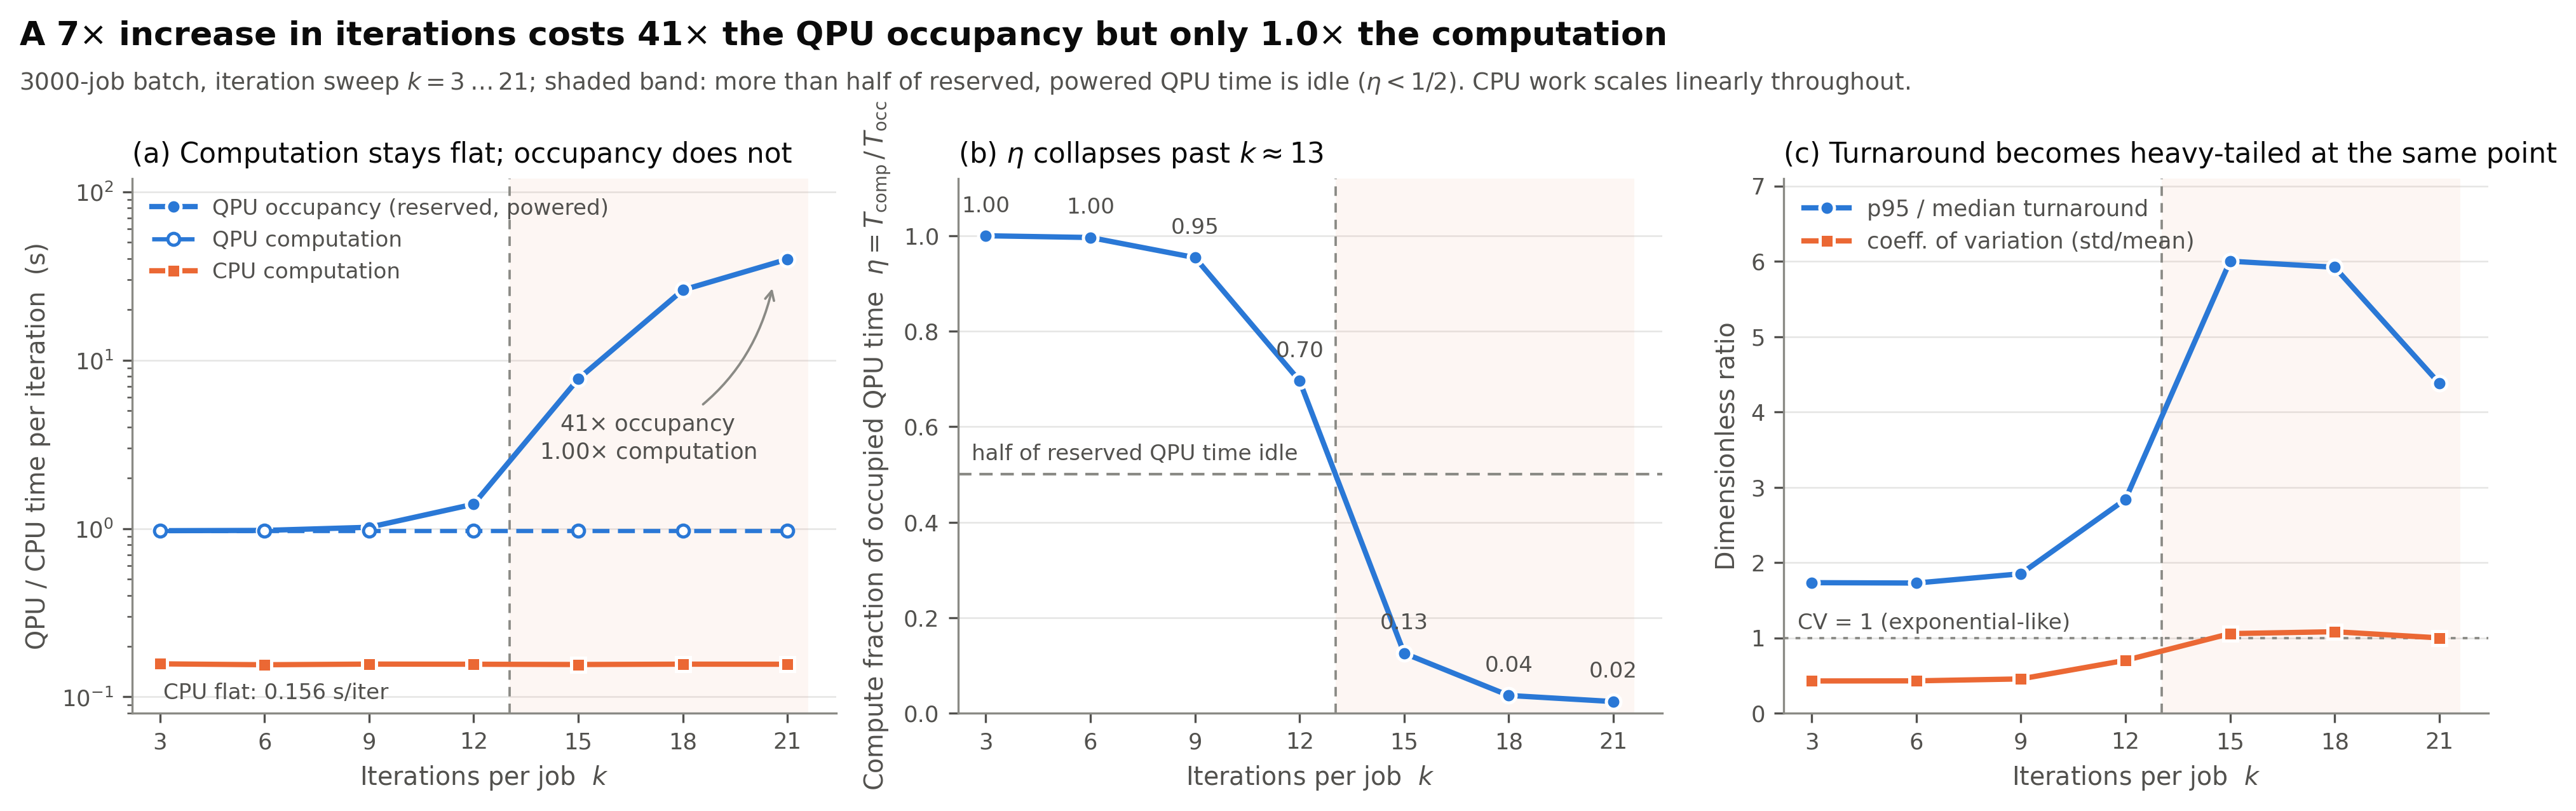
\includegraphics[width=\textwidth]{Images/Performance/plot_iteration_knee.png}
  \caption{Iteration scaling of a fixed $3000$ job variational workload on a two QPU, two CPU fleet; only $k$ varies across the seven runs. (a)~QPU time per iteration: computation is constant at \qty{0.971}{\second} while occupancy rises $41\times$; the classical phase is flat at \qty{0.156}{\second} to within $1\%$. (b)~Compute fraction of occupied QPU time, $\eta$ of Eq.~\eqref{eq:eta}; it falls through one half near $k \approx 13$ and reaches $0.024$ at $k=21$. (c)~The coefficient of variation crosses unity and the $p_{95}$/median ratio more than triples in the same bracket. The shaded band marks $\eta < \tfrac12$.}
  \label{fig:iteration-knee}
\end{figure*}

\begin{table}[t]
\centering
\caption{Iteration sweep over an identical $3000$ job trace. $\rho$ is the concurrency demand of Eq.~\eqref{eq:rho}, per iteration columns are mean phase time divided by $k$, $\eta$ is the compute fraction of Eq.~\eqref{eq:eta}, and $E$ is mean per job attributable energy. Rows below the rule lie in the shaded band.}
\label{tab:iteration-sweep}
\small
\setlength{\tabcolsep}{3.5pt}
\begin{tabular}{@{}rrrrrrrrr@{}}
\toprule
 & & \multicolumn{3}{c}{Per iteration (\unit{\second})}
 & & & \multicolumn{2}{c}{Turnaround} \\
\cmidrule(lr){3-5}\cmidrule(lr){8-9}
$k$ & $\rho$ & $T_{\mathrm{comp}}$ & $T_{\mathrm{occ}}$ & CPU & $\eta$ & $E$ (\unit{\kilo\watt\hour})
 & CV & $p_{95}/\tilde{x}$ \\
\midrule
 3 & 0.18 & 0.971 &  0.971 & 0.157 & 1.000 & 0.053 & 0.43 & 1.73 \\
 6 & 0.36 & 0.971 &  0.974 & 0.155 & 0.996 & 0.107 & 0.43 & 1.73 \\
 9 & 0.54 & 0.971 &  1.017 & 0.157 & 0.954 & 0.160 & 0.46 & 1.85 \\
12 & 0.72 & 0.971 &  1.394 & 0.156 & 0.696 & 0.213 & 0.70 & 2.84 \\
\midrule
15 & 0.90 & 0.971 &  7.727 & 0.156 & 0.126 & 0.267 & 1.06 & 6.00 \\
18 & 1.08 & 0.971 & 26.09  & 0.156 & 0.037 & 0.320 & 1.08 & 5.92 \\
21 & 1.26 & 0.971 & 39.73  & 0.156 & 0.024 & 0.373 & 1.00 & 4.38 \\
\bottomrule
\end{tabular}
\end{table}

\subsection{Results}
\label{sec:iter-results}

\paragraph{Computation is a control, and it stays flat.}
The most useful columns of Table~\ref{tab:iteration-sweep} are the two that do not move. QPU computation per iteration is \qty{0.971}{\second} at every $k$, and the measured classical phase is \qty{0.157}{\second} per iteration at $k=3$ and \qty{0.156}{\second} at $k=21$, constant to within $1\%$ across a sevenfold increase in loop length. Per job attributable energy follows, growing from $0.053$ to \qty{0.373}{\kilo\watt\hour}, a factor of $6.99$ for $7\times$ the iterations, with a QPU share flat at $98.4\%$. This is correct linear scaling measured on the same runs, which forecloses a harness artifact as the explanation for what follows.

\paragraph{The marginal iteration stops taking the same time.}
Through $k=9$ occupancy also behaves as the multiplier assumption predicts: a job holds the QPU for $0.971$, $0.974$, and \qty{1.017}{\second} per iteration. Then it breaks. Occupancy per iteration rises to $1.39$ at $k=12$, $7.73$ at $k=15$, $26.1$ at $k=18$, and \qty{39.7}{\second} at $k=21$: a $41\times$ increase in the time a job is resident on a powered QPU per iteration against a $1.00\times$ change in the time it computes there. A $21$ iteration job receives $21$ iterations that each take far longer, because the fleet is congested by jobs like itself.

\paragraph{The compute fraction collapses near $k \approx 13$.}
$\eta$ is $0.9999$ at $k=3$, $0.954$ at $k=9$, $0.696$ at $k=12$, $0.126$ at $k=15$, and $0.024$ at $k=21$, falling through one half at $k \approx 13$. Past that knee more than half, and by $k=18$ more than $96\%$, of the time a job spends resident on a cryogenically powered device is spent not computing: mean idle time per job is \qty{5.1}{\second} at $k=12$, \qty{101}{\second} at $k=15$, and \qty{814}{\second} at $k=21$, against \qty{20.4}{\second} of QPU computation. The time to drain the batch rises from \qty{2888}{\second} to \qty{4049}{\second}, and cumulative qubit utilization from $16\%$ to $89\%$.

\paragraph{Predictability collapses at the same point.}
Panel~(c) confirms this from a quantity the first two panels never touch, the shape of the turnaround distribution. Through $k=9$ turnaround is tight, with $\mathrm{CV} \le 0.46$ and a $p_{95}$ at most $1.85\times$ the median. The tail ratio reaches $2.84$ at $k=12$ and $6.00$ at $k=15$, and the CV crosses $1$ in the same bracket. The ratio narrows again at $k=21$ ($4.38$) not because the tail shortens but because the bulk has joined it: from $k=18$ to $k=21$ the median more than doubles ($267$ to \qty{574}{\second}) while the $95$th percentile grows $1.6\times$. A $k=21$ job needs \qty{23.7}{\second} of computation and waits a median of \qty{574}{\second} for it. Two quantities from different columns of the record change character in the same interval: the evidence that one mechanism is responsible.

\paragraph{The mechanism is occupancy, not work.}
Because computation is fixed, the collapse must originate in re-acquisition: a job releases its qubit region at the end of every QPU phase and re-acquires one at the next. Raising $k$ does not raise the work per iteration; it raises how long the job \emph{resides} in the system, and by Little's law a $k$ fold longer residency puts $k$ fold more jobs on the fleet at once. Concurrency demand reaches $\rho = 1$ only at $k \approx 16.6$ (Table~\ref{tab:iteration-sweep}), yet the compute fraction halves at $\rho \approx 0.78$: the knee falls while a fifth of the nominal qubit capacity is still formally free. Instrumenting the allocator shows what that gap is made of. Each blocked acquisition attempt (one second inside the phase) was classified by whether the device still held enough \emph{free} qubits for the request. At the onset of the knee, $k=12$, it did in $69.7\%$ of $14{,}963$ blocked attempts: on average $26.0$ qubits were free against $18.1$ requested, but the largest \emph{connected} free region held only $12.4$. This is connectivity fragmentation, a failure mode with no classical analogue: a heavy hex lattice that is $20\%$ free can be unable to seat an $18$ qubit circuit. As load deepens the balance shifts to plain capacity exhaustion, fragmentation accounting for $34.8\%$ of $296{,}833$ blocked attempts at $k=15$ and $14.9\%$ of $2.28$ million at $k=21$. Fragmentation initiates the collapse; saturation sustains it.

\paragraph{The energy consequence depends on what is billed.}
A superconducting QPU draws its full cryogenic baseline whenever it hosts a job, so the fleet power of Eq.~\eqref{eq:power} is paid for occupancy, computing or not. Per job energy is charged for computation only and is therefore linear in $k$: $\$0.0096$ per job at $k=3$ and $\$0.067$ at $k=21$, or $\$29$ and $\$202$ for the batch. Billing the occupied window at the same power would instead charge a $k=21$ job about $\$2.71$, roughly $1/\eta \approx 40\times$ more, and the batch about $\$8{,}100$. The difference is the cost of reserved capacity that performed no work, which under a computation based attribution falls on the facility rather than the tenant.


\subsection{Implications}
\label{sec:iter-implications}

Increasing the iteration count of a hybrid job does not make it more expensive to compute; past the knee it makes it far more expensive to \emph{hold}, and the holding dominates both the device side cost and the turnaround tail. Iteration count is therefore a \emph{capacity planning} parameter with a threshold, not a workload parameter to be optimized in isolation. An operator sizing a fleet from single job measurements at small $k$ will extrapolate linearly and under provision QPU occupancy forty fold at $k=21$, and an algorithm designer trading a longer loop for a shallower circuit may make a strictly worse system level trade even when per circuit metrics improve.


\subsection{Threats to Validity}
\label{sec:iter-validity}

Three limitations qualify these results.

First, the dispersion statistics in panel~(c) reflect variation \emph{across the $3000$ jobs within a single run} rather than replicate runs with independent random seeds. QPU computation and energy are deterministic given the trace, and an independent replicate reproduced every occupancy and dispersion statistic in Table~\ref{tab:iteration-sweep} to within $2\%$; replicate trials are still needed for confidence intervals and to resolve the knee location within the $12 \to 15$ bracket.

Second, per job energy is a sole tenant attribution: each job is charged its device's full baseline for its own computation, so per job figures cannot be summed into the facility total of Eq.~\eqref{eq:power}, and who bears the cost of idle reserved capacity is a pricing policy question the simulator exposes but does not settle.

Third, the overloaded regime ($\rho > 1$, $k \ge 18$) should be read qualitatively: turnaround there is governed by backlog drain over the finite arrival window, which is why the tail ratio recedes from $6.0$ to $4.4$ even as the median doubles. The primary result is the departure of $\eta$ from unity and its onset, not the values attained beyond it.

\section{Conclusion}
\label{sec:conclusion}

In this work, we introduce a system-level energy and cost accounting framework for hybrid quantum-classical computing. We demonstrate that job energy and cost can be systematically attributed through simulation by modeling workloads as alternating sequences of QPU and CPU execution segments, attributing consumption to execution time and macro-level device power states without requiring fine-grained hardware power models. While specific values depend on the chosen system configurations, workload patterns, and power accounting models, the framework provides a practical foundation for full-system quantum resource evaluation.

\section*{Code and Data Availability}

The source code and integrated data used for the simulations and experiments in this study are publicly accessible~\cite{SFWMSC2026}.
\section*{Acknowledgment}
This work was partially sponsored by NSF 2230111, 2238734, and 2311950.


\bibliographystyle{IEEEtran}
\bibliography{references}

% % ==========================================
% % 🔑 Call \appendix ONCE here in the main file
% % ==========================================
% \appendix
% \section*{Appendices}
% \input{Sections/Appendix-1}
% \input{Sections/Appendix-2}

\end{document}
